\documentclass{article}

% if you need to pass options to natbib, use, e.g.:
%     \PassOptionsToPackage{numbers, compress}{natbib}
% before loading neurips_2021

% ready for submission
\usepackage{neurips_2021}

% to compile a preprint version, e.g., for submission to arXiv, add add the
% [preprint] option:
%     \usepackage[preprint]{neurips_2021}

% to compile a camera-ready version, add the [final] option, e.g.:
%     \usepackage[final]{neurips_2021}

% to avoid loading the natbib package, add option nonatbib:
%    \usepackage[nonatbib]{neurips_2021}

\usepackage[utf8]{inputenc} % allow utf-8 input
\usepackage[T1]{fontenc}    % use 8-bit T1 fonts
\usepackage{hyperref}       % hyperlinks
\usepackage{url}            % simple URL typesetting
\usepackage{booktabs}       % professional-quality tables
\usepackage{amsfonts}       % blackboard math symbols
\usepackage{nicefrac}       % compact symbols for 1/2, etc.
\usepackage{microtype}      % microtypography
\usepackage{xcolor}         % colors

% custom packages
\usepackage{amsmath}
\usepackage{amssymb}
% for referencing footnotes several times. to load after hyperref
\usepackage{cleveref}
\crefformat{footnote}{#2\footnotemark[#1]#3}
\usepackage{caption}
% table positioning
\usepackage{placeins}
\usepackage[pdftex]{graphicx}
% interval
\newcommand{\interval}[2]{\mathopen{[}#1\,;#2\mathclose{]}}

\renewcommand{\floatpagefraction}{.95} %avoid big figure to get it's own float page
\setlength{\belowcaptionskip}{-18pt}  % reduce space below caption
\usepackage[compact]{titlesec} % compact layout
\def\permille{\ensuremath{{}^\text{o}\mkern-5mu/\mkern-3mu_\text{oo}}}

\title{Joint self-supervised blind denoising and noise estimation}

% The \author macro works with any number of authors. There are two commands
% used to separate the names and addresses of multiple authors: \And and \AND.
%
% Using \And between authors leaves it to LaTeX to determine where to break the
% lines. Using \AND forces a line break at that point. So, if LaTeX puts 3 of 4
% authors names on the first line, and the last on the second line, try using
% \AND instead of \And before the third author name.

\author{%
  Jean Ollion\thanks{www.sabilab.fr}\\
  SABILab, France\\
  \texttt{jean.ollion@polytechnique.org} \\
  \And
  Charles Ollion\\
  CMAP, Ecole Polytechnique, Institut Polytechnique de Paris, France\\
  \And
  \'Elisabeth Gassiat\\
  Universit\'e Paris-Saclay, CNRS, Laboratoire de math\'ematiques d'Orsay, 91405, Orsay, France\\
  \And
  Luc Leh\'ericy\\
  Laboratoire J. A. Dieudonn\'e, Universit\'e C\^ote d'Azur, CNRS, 06108, Nice, France\\
  \And
  Sylvain Le Corff \\
  CMAP, Ecole Polytechnique, Institut Polytechnique de Paris, France\\
  Samovar, T\'el\'ecom SudParis, D\'epartement CITI, Institut Polyechnique de Paris, France\\
  \texttt{sylvain.le_corff@telecom-sudparis.eu} \\
}

\begin{document}

\maketitle

\begin{abstract}
We propose a novel self-supervised image blind denoising approach in which two neural networks jointly predict the clean signal and infer the noise distribution.
Assuming that the noisy observations are independent conditionally to the signal, the networks can be trained jointly without any clean data. This approach is particularly relevant for biomedical image denoising where the noise is difficult to model precisely and clean training data are usually unavailable. Our method significantly outperforms current state-of-the-art self-supervised blind denoising algorithms on six publicly available biomedical image datasets, as well as its supervised counterpart. We also show empirically that it is able to capture noise distributions efficiently, both on different synthetic noise models and real multimodal and skewed data.
Finally, the described framework is simple, lightweight and computationally efficient, making it useful in practical cases.
\end{abstract}

\section{Introduction}
\label{sec:introduction}

Image denoising is a well-known Computer Vision task designed to restore pictures taken in poor conditions. In scientific imagery (microscopy, astronomy, etc.) for instance,  the optical setting may produce very noisy images, which limits their interpretability or their automatic processing.
Formally, image denoising is the process of recovering a clean signal $X$ given an observation $Y$ corrupted by an additive noise $\varepsilon$. Classical denoising approaches are model-driven in the sense that they rely on strong assumptions on the noise distribution or on the structure of the signal but are often limited by the relevance of these assumptions.
Recently, efficient data-driven methods have emerged. Most of them assume that pairs made of noisy data $Y$ associated with a clean signal $X$ are available in a supervised learning framework, see for instance \cite{weigert2017content}. In \cite{lehtinen2018noise2noise}, the authors have demonstrated that it is possible to train an efficient denoising method using only pairs of independent noisy measurements $(Y^1, Y^2)$ of the same signal. Such assumptions have also been used to solve deconvolution problems with repeated measurements as in \cite{delaigle2008deconvolution}. However, obtaining independent observations of the same signal is often unrealistic in practice.

Recent self-supervised methods have overcome this limitation \cite{batson2019noise2self,krull2018noise2void} by training a neural network to predict the value of a (corrupted) pixel $Y$ only using the noisy observations of the surrounding pixels. In such frameworks, the trained network extracts some local structure in the signal and therefore can be used as a denoiser. Such approaches are referred to as \textit{blind-denoising} as they only assume that the noises associated with different observations are independent and centered.
This is well suited to typical microscopy settings, in which the clean image is unavailable and the noise process is complex and not known.

These methods rely on training a function $f_\theta$ depending on an unknown parameter $\theta$, usually implemented as a convolutional neural network. Using only the noisy observations and a binary mask $M$, the objective is to minimize a self-supervision loss of the form $\theta\mapsto \sum_{i=1}^N \|f_\theta(Y^{masked}_i) - Y_i\|_2^2$,
where $Y^{masked}_i$ is an image in which the pixel $Y_i$ has been masked using $M$. This masking step is crucial to foster learning of local structure in the signal to predict the masked values.

While these methods are appealing in practice and result in efficient denoising functions, they suffer from several drawbacks:
1/ it is not well understood why they are so effective in practice, i.e. what type of noise they are able to remove, and how sensible they are to the masking scheme for instance;
2/ they often suffer from high frequency denoising artifacts known as \textit{checkerboard pattern}.

To address these issues, we introduce a novel self-supervised method, based on the joint training of two neural networks referred to as D-net (denoiser net) and N-net (noise net). Similar to previous works, the denoiser is a convolutional neural network and receives a masked input during training.
Our main contribution is to add the flexible N-net which recovers precisely the noise distribution during training, even for complex asymmetric noises.
We derive this method from a novel mathematical modeling of the denoising problem, opening new avenues for better understanding of why self-supervised networks achieve remarkable results.

The contribution of this work can be summarized as follows:
1/ we introduce a novel self-supervised blind-denoising method, modeling both the signal and the noise distributions;
2/ we show that the N-net recovers the noise distribution efficiently in varying experiments with synthetic and real noises;
3/ the proposed architectures outperform state-of-the-art algorithms over 6 standard microscopy datasets, without introducing denoising artifacts.

\section{Related work}
\label{sec:related}
\paragraph{Masking and J-invariance.}
The most typical class of denoising functions is chosen to be comprised of convolutional neural networks (CNNs), which are heavily parameterized functions and are not restricted to solve denoising problems. As an important consequence, a naive self-supervised loss without any masking would result in learning the identity function (i.e. the function outputing the noisy observation $Y$ if it is not masked in the input data), as the considered CNNs can typically implement it. Starting from this intuition, many of the related works can be viewed as different masking schemes. This has been described in the \textit{J-invariant} framework introduced by \cite{batson2019noise2self}: a \textit{J-invariant} function does not depend on a few selected dimensions $J$ of its input variables; typically this translates into a convolutional function which does not depend on the central pixel of the convolutional receptive field, but rather on the observations of neighboring pixels\footnote{Those functions excluding the central pixel are sometimes also called \textit{blind spot}, not to be confused with \textit{blind denoising} in which the noise process is not known.}.

The first masked self-supervised denoising methods were introduced by Noise2Void (N2V) \cite{krull2018noise2void}, in which $\{(Y^{masked}_i,Y_i)\}_{1\leqslant i\leqslant N}$ are sampled randomly in the picture, and masking consists in replacing $Y_i$ by a random observed value in its neighborhood, with a positive probability of replacing $Y_i$ by itself meaning that leaks in masking are introduced.

Noise2Self (N2S) \cite{batson2019noise2self} masking procedure differs from N2V in the sense that $\{(Y^{masked}_i,Y_i)\}_{1\leqslant i\leqslant N}$ are obtained with a fixed grid, and $Y_i$ is replaced by the average of the 4 direct neighboring observations.
In practice, the masking procedure has a strong impact on training: (i) improving masking schemes can improve denoising performance and (ii) as only masked pixels are used for training, typically representing a few percent of the image, this affects greatly the training efficiency.

The underlying CNN architecture implemented by these works is the U-net \cite{ronneberger2015u}, a typical convolutional autoencoder architecture, involving skip connections, which can reproduce fine grained details, while making use of higher-level spatially coarse information. While showing strong denoising performance in N2S and N2V, they however can produce \textit{checkerboard patterns}, which are high frequency artifacts that arise in the denoised results.
These works have been extended in DecoNoising \cite{goncharova2020} in which a Gaussian convolution is added after the neural network output to simulate microscope Point Spread Function.
This technique improves performances, however the deconvolved image (predicted image before the Gaussian convolution) displays even stronger checkerboard pattern.

Finally, \cite{broaddus2020removing} showed that when the noise has local correlations (for instance a  directional noise),  masking can be adapted to remove them - by masking adjacent pixels in the same direction as the noise spatial correlation for instance.

\paragraph{J-invariance without masking.}
Instead of masking specific pixels, it is possible to design specific convolutional operators to limit the receptive field, ensuring that the resulting function is \textit{J-invariant} by design. This was achieved in \cite{laine2019high} by introducing directional convolution kernels, each kernel has its receptive field restricted to a half-plane that does not contain the central pixel. The associated function then takes values which only depend on pixels in specific directions, ensuring that it does not depend on pixels in the opposite direction. One drawback is that the inference has to be performed four times, one in each direction.

More recently, \cite{lee2020noise2kernel} introduced a combination of specific convolution operators with dilation and strides, guaranteeing that the function is independent of the central pixel by design, therefore \textit{J-invariant}. It is interesting to note that with standard convolutions, a two layered network already cannot be made independent of the central pixel, which is why the authors had to rely on very specific convolutions.

The benefit of these architectures compared to the masking-based training is that all output pixels can contribute to the loss function as in conventional training, rather than just the masked pixels; and they do not require a carefully tuned masking procedure. However, they strongly constrain the network architecture, which can hinder the denoising performance or result in more expensive inference schemes.

\paragraph{Contribution of a noise model.}
The denoising literature includes few works which explicitly model the noise distribution, either by choosing \textit{a priori} a  family of distributions (e.g. a Gaussian noise), or by selecting a more flexible class of distributions.

The former is illustrated in \cite{laine2019high}, in which three types of corrupting noise are considered: Gaussian noise independent of the signal; Poisson-Gaussian noise, i.e. a Gaussian noise with variance scaling linearly with the signal value; finally impulse noise, i.e. a uniform noise. In each case, the noise parameters are either known or estimated with an auxiliary neural network. As the signal distribution and the noise distribution belong to a known parametric family, the noisy central pixel can be included at test time in order to improve performances. However, as the noise type has to be chosen \textit{a priori}, the method is restricted to known and synthetic noise types and therefore falls under the category of \textit{non-blind denoising} methods.

In \cite{krull2019probabilistic,prakash2020fully}, the authors make use of a more flexible noise model, which is a generic modelisation of the conditional distribution of the noise given the signal intensity and thus can better model real noises.
%: $p(y|x) = N(x): \mathbb{R} \to \mathbb{R}$,
In these works, noise models are approximated using 2D histograms of denoised and noisy observed values, either using additional calibration data (in that case the method is not fully self-supervised) or using a previously trained denoising function \cite{prakash2020fully}.
In the latter variant, the noise distribution is parametrized with a centered Gaussian mixture model with empirically designed constraints.
This increases the complexity of the method, as it requires several training procedures and calibration.
% The denoising network is then trained to predict a whole distribution of $800$ possible noisy values instead of a single point estimate of each pixel, approximating the previously defined noise distribution at each pixel.
\cite{2020DivNoising} used the Variational Auto\-Encoder formalism, adding a noise model in their architecture.
This provides new interesting possibilities, as it can generate a diversity of denoised results, possibly interesting in creative processes.
In the case of scientific images such as microscopy, the possible presence of visual artifacts or blurry results makes it less appropriate.
The authors address co-learning of a noise model by constraining noise variance to scale linearly with the signal value, which corresponds to assuming a Poisson-Gaussian noise distribution, and thus makes the method not blind.

It is worth noting that supervised \textit{blind denoising} methods have used parametrized noise models, such as \cite{zhang2017beyond,yue2019variational}, which explicitly used large neural networks to model a complex noise, with even less assumptions (it can be slightly structured). Even though the algorithm proposed in \cite{yue2019variational} is able to train jointly a noise network and a denoiser, their modeling only works in a supervised setting, which does not apply in our setting.

\paragraph{Chosen approach.} The work of Laine et al. \cite{laine2019high} gave the intuition that a strictly J-invariant function lacks the information of the central pixel at test-time. On the contrary, methods such as N2V or N2S use the central pixel at test-time, but the dependency on the central pixel is not explicit and unknown. Instead of focusing on finding new strictly \textit{J-invariant} functions at test time, our approach rather emphasizes on designing an efficient masking procedure only at train-time. Our mathematical formulation enables the use of the central pixel at test time.
This also gives the flexibility to tune the masking to match structured noises, which we observed in 2 of the 6 considered datasets (see section~\ref{sec:masking}).
We also build upon the work of \cite{laine2019high, krull2019probabilistic} by designing a noise model which can be jointly trained alongside the denoiser (see Fig.~\ref{fig:plumbing}), and only requiring a single prediction per pixel: this results in a training and inference procedures that are simpler, more efficient and more stable.

\section{Model}
\label{sec:model}

Estimating a signal corrupted by additive noise  is a challenging statistical problem. In such frameworks, the received observation $Y$ is given by $Y = X + \varepsilon$,  where $X$ is the signal and $\varepsilon$ is the noise. A lot of works have been devoted to deconvolution where the aim is to recover the distribution of the signal based on the observations. It has been for instance applied in a large variety of disciplines and has stimulated a great research interest in signal processing \cite{moulines1997maximum,attias1998blind}, in image reconstruction \cite{kundur1996blind,campisi2017blind}, see also  \cite{meister:2009}. Recently, \cite{gassiat:lecorff:lehericy:2021} proved that it is possible to recover the signal distribution when $X$ has at least two dimensions and may be decomposed into two subsets of random variables which satisfy some weak dependency assumption. This identifiability result does not require any assumption on the noise distribution but illustrates that the components of the signal must be dependent to allow its identification. %The results proposed in \cite{gassiat:lecorff:lehericy:2021} motivate the denoising approach introduced in this work where several classes of noises are considered to describe the observations received from the target signal.  %The signal $X$ is modeled as a function of the noisy observation $Y$ and its neighborhood $\Omega_Y$: $X =  \mu_{\theta_p}(\Omega_Y;Y)$.

In this work, it is assumed that the observation $Y$ associated with $X$  is given by
%\begin{equation}
%\label{eq:def:Y}
%Y = X + \sigma_{\theta_n}(X)\varepsilon\,,
%\end{equation}
\begin{equation}
\label{eq:def:Y}
Y = X + \varepsilon\,,
\end{equation}
%which means that
%$$
%Y = X + (\mu_{\theta_p}(\Omega_Y;\overline{\Omega_Y})-\mu_{\theta_p}(\Omega_Y;Y)) + \sigma_{\theta_n}(\mu_{\theta_p}(\Omega_Y;\overline{\Omega_Y}))\varepsilon
%$$
%The blind denoising framework introduced in this work can be written as a regression problem where the observations conditionally on $\Omega_Y$ the observation is given by
%$$
%Y = \mu_{\theta_p}(\Omega_Y;\overline{\Omega_Y}) + \sigma_{\theta_n}(\mu_{\theta_p}(\Omega_Y;\overline{\Omega_Y}))\varepsilon\,,
%$$
%where $\varepsilon$ is a centered noise  independent of $X$ and $\sigma^2_{\theta_n}$ is parameterized by a convolutional neural network, called N-net and with unknown weights $\theta_n$.
%This contrasts with most common denoising algorithms where $\varepsilon$ is assumed to be a centered Gaussian random variable and  $x\mapsto \sigma^2_{\theta_n}(x)$ is either known and constant or has a Poisson-Gaussian shape i.e., scales with $\alpha x + \eta^2$.
%As illustrated in Section~\ref{sec:results}, these assumptions do not usually hold, in particular when considering biomedical images, and they may have a severe impact on denoising performances.
where $\varepsilon$ is a centered noise. In this paper, it is assumed that $\varepsilon$ has a mixture distribution with signal-dependent weights, means and variance:
$$
\varepsilon \sim \sum_{k=1}^N \alpha_k(X)\varphi_{\mu_k(X),\sigma_k^2(X)}\,,
$$
where $\varphi_{\mu,\sigma^2}$ is the Gaussian probability density function with mean $\mu$ and variance $\sigma^2$, $(\alpha_k(X))_{1\leqslant k\leqslant N}$ are nonnegative real numbers with $\sum_{k=1}^N\alpha_k(X) = 1$, and $\{(\mu_i(X),\sigma_i^2(X))\}_{1\leqslant k\leqslant N}$ are  parameterized by a convolutional neural network, called N-net and with unknown weights $\theta_n$.
This contrasts with most common denoising algorithms where $\varepsilon$ is assumed to be a centered Gaussian random variable and with a variance which is either known and constant or has a Poisson-Gaussian shape i.e., scales with $\alpha x + \eta^2$.
As illustrated in Section~\ref{sec:results}, these assumptions do not usually hold, in particular when considering biomedical images, and they may have a severe impact on denoising performances.



 %while  model \eqref{eq:def:Y} is shown to be robust to real noise distributions.
%Our model does not fit directly the assumptions of
In \cite{gassiat:lecorff:lehericy:2021}, the variance of the noise is assumed to be constant and the target signal is assumed to be weakly dependent to obtain identifiability of the noise and the signal  distributions. % remains an open problem in this setting.
%In \cite{gassiat:lecorff:lehericy:2021}, the signal is assumed to be multivariate with  $\sigma^2_{\theta_n}$ independent of $X$.
%However, our approach in this work is motivated by the fact that $\varepsilon$ is independent of $X$ and that $X$ depends on its neighborhood.
%Conditionally to $X$, we propose a more general corrupting process as $\varepsilon$ is a centered Gaussian random variable with variance $\sigma^2_{\theta_n}(X)$ where $\sigma^2_{\theta_n}$ is parameterized by a convolutional neural network, called \textit{N-net} and with unknown weights $\theta_n$.
%We also propose an extension of this setting in which $\varepsilon$ is a mixture of Gaussian random variables with state-dependent variances to account for skewness.
In \eqref{eq:def:Y}, we extend the model  proposed by \cite{gassiat:lecorff:lehericy:2021} by considering a state-dependent standard deviation and identifiability remains an open problem. However, we assume in this work that $X$ is dependent with the signal in the neighbooring pixels $\Omega_X$ so that heteroscedasticity is the only challenge to obtain identifiability of \eqref{eq:def:Y} which is left for future works.
In this work, we assume that $(X,\Omega_X)$ is a random vector with dependent variables and we propose to model the conditional mean of $X$ given $(Y,\Omega_Y)$ by a parametric function denoted by $\mu_{\theta_d}$ so that $\mathbb{E}[X|Y,\Omega_Y] = \mu_{\theta_d}(\Omega_Y,Y)$ where $\Omega_Y$ are the noisy observations of the signals in the neighborhood of $X$. The function $ \mu_{\theta_d}$ is parameterized by a convolutional neural network, called D-net and with unknown weights $\theta_d$.

A natural estimator of $X$ given the noisy observations is $\widehat X = \mu_{\theta_d}(\Omega_Y,Y)$.
During training this predictor $\widehat X$ cannot be used to estimate $\theta_d$ and $\theta_n$ as $\mu_{\theta_d}$ would learn to output the noisy observation $Y$ if it is not masked in the input data.
This is the reason why we adopt a making approach and assume during training that $\mu_{\theta_d}$ cannot use $Y$ as an input which must be replaced by an estimator.
In this framework, a genuine prediction of $Y$ is given by $\mathbb{E}[Y|\Omega_Y]$ which we estimate by $\mu_{\theta_d}(\Omega_Y,g(\Omega_Y))$ where $g$ is a known function. %In the experiments below, we chose to set $g(\Omega_Y)$ as the empirical mean of the noisy pixels in $\Omega_Y$.
In the experiments below, we provide empirical evaluations that choosing $g(\Omega_Y)$ as the empirical mean of the noisy pixels in $\Omega_Y$ is a robust solution while other choices can be made straightforwardly.

%The signal $X$ is then modeled as
%\begin{equation}
%\label{eq:def:X}
%X =  \mu_{\theta_p}(\Omega_X,U)\,,
%\end{equation}
%where $\Omega_X$ are the signal values in a neighborhood of $X$ and $U$ is a random variable on $\mathbb{R}$. % $\Omega_X$-measurable.
% In the case where the random variable $U$ is $\Omega_X$-measurable, there exists a measurable function $g$ such that $U = g(\Omega_X)$.
%Combining this with the additive model  \eqref{eq:def:Y} yields the following loss function associated with $N$ observations $(Y_1,\ldots,Y_N)$:
%$$
%\ell_{\theta}: (Y_1,\ldots,Y_N) \mapsto \frac{1}{N}\sum_{i=1}^N \ell_{\theta}(Y_i|\Omega_{Y_i})\,,
%$$
%where $\theta = (\theta_n,\theta_d)$ and
%\begin{multline*}
%\ell_{\theta}(Y_i|\Omega_{Y_i}) = \log(\sigma_{\theta_n}( \mu_{\theta_d}(\Omega_{Y_i},g(\Omega_{Y_i})))^2) \\
%+ \left(\frac{Y_i-\mu_{\theta_d}(\Omega_{Y_i},g(\Omega_{Y_i}))}{\sigma_{\theta_n}(\mu_{\theta_d}(\Omega_{Y_i},g(\Omega_{Y_i}))}\right)^2\,. %\frac{(Y_i-\mu_{\theta_p}(\Omega_{Y_i};\overline{\Omega_{Y_i}}))^2}{\sigma_{\theta_n}(\mu_{\theta_p}(\Omega_{Y_i};\overline{\Omega_{Y_i}}))^2} \,,
%\end{multline*}
%This loss is obtained by computing the conditional loglikelihood of $Y$ given $X$ evaluated at the predictor of $Y$ obtained by replacing $\Omega_{X}$ by the observed values $\Omega(Y)$ in \eqref{eq:def:X}.
Combining this with the additive model  \eqref{eq:def:Y} yields the following loss function associated with $n$ observations $(Y_1,\ldots,Y_n)$:
$$
\ell_{\theta}: (Y_1,\ldots,Y_n) \mapsto \frac{1}{n}\sum_{i=1}^n \ell_{\theta}(Y_i|\Omega_{Y_i})\,,
$$
where $\theta = (\theta_n,\theta_d)$ and
$$
\ell_{\theta}(Y_i|\Omega_{Y_i}) = \log\left(\sum_{k=1}^N\frac{\alpha_k(\mu_{\theta_d}(\Omega_{Y_i},g(\Omega_{Y_i})))}{\sqrt{2\pi }\sigma_{\theta_n}(\mu_{\theta_d}(\Omega_{Y_i},g(\Omega_{Y_i}))}\exp\left\{-\frac{1}{2}\left(\frac{Y_i-\mu_{\theta_d}(\Omega_{Y_i},g(\Omega_{Y_i}))}{\sigma_{\theta_n}(\mu_{\theta_d}(\Omega_{Y_i},g(\Omega_{Y_i}))}\right)^2\right\}\right)\,.
%\log(\sigma_{\theta_n}( \mu_{\theta_d}(\Omega_{Y_i},g(\Omega_{Y_i})))^2) \\
%+ \left(\frac{Y_i-\mu_{\theta_d}(\Omega_{Y_i},g(\Omega_{Y_i}))}{\sigma_{\theta_n}(\mu_{\theta_d}(\Omega_{Y_i},g(\Omega_{Y_i}))}\right)^2\,. %\frac{(Y_i-\mu_{\theta_p}(\Omega_{Y_i};\overline{\Omega_{Y_i}}))^2}{\sigma_{\theta_n}(\mu_{\theta_p}(\Omega_{Y_i};\overline{\Omega_{Y_i}}))^2} \,,
$$

An interesting  feature of our approach is that it can be extended straightforwardly to more complex noise distributions. As detailed above, model \eqref{eq:def:Y} is an extension of the model considered in \cite{gassiat:lecorff:lehericy:2021} where the authors establish that the noise distribution can be identified without any assumption. Full identifiability of model \eqref{eq:def:Y} remains an open question but we display in Section~\ref{sec:experiments} an example of non-Gaussian noises, and we propose an application with mixture models  to account for positive skewness which cannot be modeled with a single Gaussian distribution. In this context, each component of the mixture describing the distribution of $\varepsilon$ is a Gaussian distribution with signal-dependent standard deviation. The results provided in Section~\ref{sec:experiments} illustrate how such models improve denoising performance for asymmetrical noise distributions.
%The random variable $U$ being  $\Omega_X$-measurable, there exists a measurable function $g$ such that $U = g(\Omega_X)$

%After a training phase to estimate $\theta$, the signal values cannot be predicted as the random variable $U$ is not observed. Several predictors of $X$ can be designed.



%uses the fact that by \eqref{eq:def:X} $Y_i$ is a natural linear predictor of $X_i$ and then
%instead of introducing an explicit noise  distribution in the definition of $U$ and  therefore in \eqref{eq:def:X} and then to estimate the posterior distribution of $X$ given $Y$ we propose to introduce a loss function which

% and $\overline{\Omega_Y}$ is the empirical mean of $\Omega_Y$.
%The approach proposed in this work is decomposed into two steps.
%\begin{enumerate}
%\item First, $\mu_{\theta_p}$ is obtained with the P-Net fed with $\Omega_y$ and $\overline \Omega_y$ at central position, $\sigma_{\theta_n}^2$ is  obtained with the N-Net fed with $\mu_{\theta_p}$.
%\item After a training procedure to estimate the parameters of these networks, the estimator of the unknown pixel given the observations $(y,\Omega_y)$ is set to $\mu_{\theta_p}(\Omega_y,y)$ as an approximation of the posterior mean.
%\end{enumerate}
%The signal $X$ is then modeled as $X =  \mu_{\theta_p}(\Omega_Y;Y)$ so that
%$$
%Y = X + \Delta_{\theta_p}(\Omega_Y;\overline{\Omega_Y},Y) + \sigma_{\theta_n}(\mu_{\theta_p}(\Omega_Y;\overline{\Omega_Y}))\varepsilon\,,
%$$
%where
%\begin{align*}
%\Delta_{\theta_p}(\Omega_Y;\overline{\Omega_Y},Y)  &=  \mu_{\theta_p}(\Omega_Y;\overline{\Omega_Y})  -\mu_{\theta_p}(\Omega_Y;Y) \,,\\
%&\sim \partial_2\mu_{\theta_p}(\Omega_Y;Y)[\overline{\Omega_Y}-Y]
%\end{align*}


\section{Experiments}
\begin{figure}[!htbp]
\vskip -0.1in
\begin{center}
\centerline{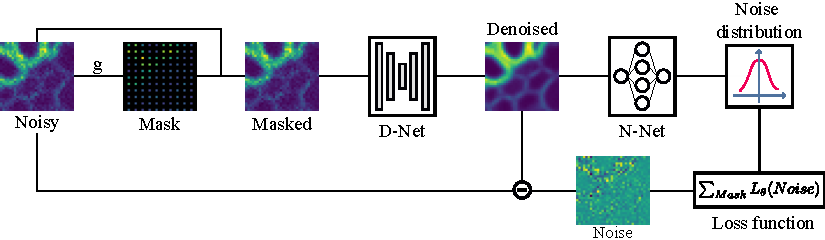
\includegraphics[width=\columnwidth]{fig_plomberie_1col.pdf}}
\caption{Training setup.
For each mini-batch, a random grid is drawn.
The masking function $x\mapsto g(x)$ is applied on each element of the grid, replacing the original pixels in the masked image.
The denoised image predicted by the D-net is fed to the N-net that predicts a noise distribution for each pixel.
The loss function is then computed on each element of the grid.
}
\label{fig:plumbing}
\end{center}
\end{figure}

\label{sec:experiments}
\subsection{Model Architecture}
\paragraph{D-net.}
The function $\mu_{\theta_d}$ is parametrized by a U-net. The main difference with the networks used in N2S and N2N is that we use upsampling layers with nearest-neighbor approximation instead of transpose convolutions ---as we observed that transpose convolution tends to increase the checkerboard artifact--- directly followed by a 2x2 convolution to enable trainable upsampling.
Additional architecture and training information can be found in section~\ref{si:implementation}.
The receptive field of this network is 35x35 pixels, which means that the network may use pixels from the neighborhood that are masked.
At test-time, we averaged the prediction of the image with the predictions of its transposed and flipped versions on each axis, which improves performances.

\paragraph{N-net.}
The function $\sigma_{\theta_n}: \mathbb{R} \to \mathbb{R}$ describing the local variance of the noise distribution is a fully-connected deep neural network with several hidden layers. This choice is motivated by the large expressivity of such a network, necessary to approximate complex noise distributions. In practice, it is applied to each pixel, so it is implemented efficiently as a fully convolutional network using only 1x1 convolutional layers. In the Gaussian Mixture Model (GMM) case, the network parametrizes a more complex distribution and therefore has several outputs: for a mixture of $N$ Gaussian distributions, there are $N$ variances, $N-1$ means (the last mean is computed to ensure that the resulting distribution is centered) and $N$ mixture weights parametrized by the N-net. The full architecture detail for both models are available in section~\ref{si:implementation}.

%This choice is motivated by the fact that such networks can be trained in a supervised way with a clean image $X$ as input and the following cost function, where $Y$ is a corrupted observation of $X$ \textcolor{red}{il faut l'llustrer dans les supplementary non ?}:$y\mapsto\varphi_{0,\sigma_n^2}(x)$.
%The essential aspect of the architecture is that the network contain no spatial convolution (only 1x1 convolutions), otherwise the noise distribution is not well described by the network. This is consistent with our model, in which the noise is independent of the neighborhood.

\subsection{Datasets}
\label{sec:datasets}
We train and evaluate our method on 6 publicly available datasets of microscopy images. In those datasets, ground truth ($X$) is estimated by averaging several observations ($Y$) of the same field-of-view (FOV).
This allows to have access to an estimation of the noise $Y-X$, which we refer to as \textit{real noise} in this article.

The 3 first datasets (\emph{PN2V-C}, \emph{PN2V-MN}, \emph{PN2V-MA}) have been published along with the PN2V method \cite{krull2019probabilistic}, each is composed of several observations of one single FOV.
For a fair comparison, we use the same training and evaluation sets as the authors: for each sample type the whole dataset is used for training, and only a subset of the FOV is used for evaluation (see section~\ref{si:datasetxp} for details).
The 3 last datasets are the 3 channels of the W2S dataset \cite{zhou2020w2s} referred to as \emph{W2S-1}, \emph{W2S-2} and \emph{W2S-3}.
The dataset is composed of 120 FOV, the first 80 are used for training and the last 40 for evaluation (see section~\ref{si:datasetxp} for more details).
Following the authors, for each FOV, only one observation is used for training and for evaluation, which better corresponds to a real setting where only one observation per FOV is available.

\subsection{Masking procedure}
\label{sec:masking}
Following \cite{batson2019noise2self}, we mask pixels along a grid and compute the loss only on masked pixels.
We obtained the best results by replacing the central value by the weighted average of the 8 direct neighbors with Gaussian weights ($\sigma=1$).
The drawback of masking along a grid is that pixels are masked at fixed relative positions with regards to the central pixel.
If grid spacing is too small, then too many masked pixels are present in the receptive field and perturb the performances, because the available information is reduced.
On the other hand, the larger the spacing, the less pixels are used for training, which reduces dramatically training efficiency.
In order to push the limits of this trade-off, we use a random dynamic spacing between 3 and 5 pixels, which allows to have relative positions of masked pixels that change randomly.
On average, $6.8\%$ of the image is masked.

Furthermore, we observed that datasets \emph{PN2V-C} and \emph{PN2V-MA} display axial correlation in the noise, for those datasets we adapted the masking procedure introduced in \cite{broaddus2020removing}: the replacement value was computed on a neighborhood excluding the neighbors along the correlation axis, and neighbors were masked along this axis, within an extent of 3 pixels. This can be determined easily in a self-supervised setup because the neural network tends to amplify the noise correlation.

\subsection{Training}
\label{sec:training}
Networks are trained using Adam optimizer with a learning rate of $4\cdot10^{-4}$, decreased by $1/2$ on plateau of 30 epochs until $10^{-6}$. We train networks for 400 epochs of 200 steps.
Training time is about 2 min per epoch on a NVIDIA Tesla P4.
We obtain better and more reproducible results using the weights of the trained model at the last epoch instead of the weights of the model with the best validation loss, possibly because the loss is a bad proxy for the denoising performances. For that reason, we do not use a validation step.
Batch size is set to 1, and each batch is split into 100 (overlapping) tiles of 96x96 pixels.
Tiles are augmented with random horizontal and/or vertical flip and/or a random rotation with an angle chosen within $(90^\circ, 180^\circ, 270^\circ)$, except for datasets with axial noise correlation where axes transpositions are avoided.

\subsection{Evaluation}
We compared denoised image to ground truth with the classical Peak Signal-to-Noise Ratio (PSNR) metric.
However PSNR is not highly indicative of perceived similarity, in particular it does not reflect similarity of high frequency information such as textures and local contrasts \cite{wang2004image}, that denoising methods tend to reduce. It is thus essential to have other metrics that them into account.
To address this shortcoming, we used Structural Similarity (SSIM) that take textures and edges into account \cite{wang2004image}, computed as in the original work.

\section{Results}
\label{sec:results}
\subsection{Noise estimation}

\paragraph{Estimation on synthetic noise.}
To evaluate the capacity of the N-net to capture blindly different noise distributions, we generated 3 datasets by adding synthetic noise to the ground truth of dataset \textit{W2S-1}, and we chose the parameters of the noise models so that PSNR of noisy images match the one of the original dataset (in a range of $\pm0.1$dB).
We used 3 classical noise models: additive Gaussian, Poisson-Gaussian (which is a good model for shot noise) and speckle (see section~\ref{si:synthetic} for details).
Empirical and predicted distributions of the noise standard deviation are illustrated in Fig.~\ref{fig:noisestd}.
One of the most striking result of this experiment is that for the 3 cases of synthetic noise, the predicted standard deviation provided by the N-net is a very sharp approximation of the known theoretical standard deviation.
It shows in particular that our method is able to capture the different noise distributions even in areas where signal is rare.
\begin{figure}[!htbp]
\vskip -0.1in
\begin{center}
\centerline{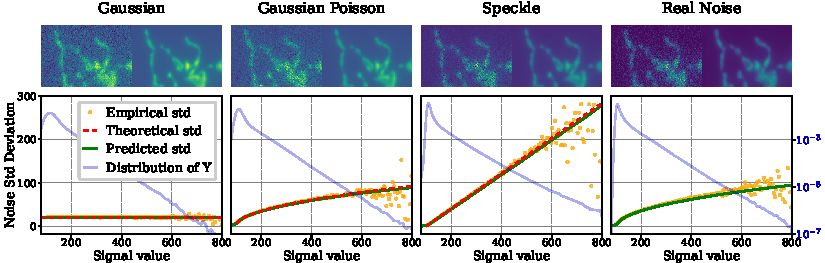
\includegraphics[width=\textwidth]{fig_noise_std_1col.pdf}}
\caption[Noise estimation]{Noise estimation.
For 3 models of synthetic noise as well as the real noise, the plots display the empirical standard deviation of the noise $Y - X$, as well as the predicted standard deviation of the noise by the N-net as a function of $X$ (Note that display range was shrinked in Y-axis for visualization purposes.).
Theoretical standard deviation of the noise is displayed for the 3 models of synthetic noise.
The empirical distribution of $Y$ is displayed in blue, in logarithmic scale.
Examples of noisy images corrupted with the corresponding noise model and the predicted denoised images are displayed above each graph.}
\label{fig:noisestd}
\end{center}
\end{figure}

\label{sec:exp:real:noise}
\paragraph{Improving estimation on real noise.}
We observed that contrary to the classical noise models considered in the denoising literature, real noise often displays a certain amount of skewness, as illustrated in Fig.~\ref{fig:skewness}.
In order to be able to capture this aspect, we predict a Gaussian mixture model (GMM) instead of a simple Gaussian model as described in Section~\ref{sec:model}. Fig.~\ref{fig:skewness} shows that noise skewness is well described by the predicted model, and the noise distribution is better described by a GMM than by a single Gaussian.
This applies for all datasets and the equivalent figures can be found in section~\ref{si:skewness}.
In this example, it is interesting to note that the Kullback–Leibler divergence between the empirical noise distribution and the predicted distribution (as a function of the signal value) is improved by considering a GMM instead of a unimodal distribution.
This supports the use of our flexible N-net to capture a large variety of noise distributions (with multimodality and/or skewness) which can be observed in experimental datasets.
This comment paves the way to several perspectives for our work such as the design of statistically consistent model selection procedures to choose automatically the number of mixing components.
Such approaches have been proposed in more simple cases using for instance penalized maximum likelihood based algorithms.
This remains an open problem in our framework and we leave this topic for future research.
\begin{figure}[!htbp]
\vskip -0.1in
\begin{center}
\centerline{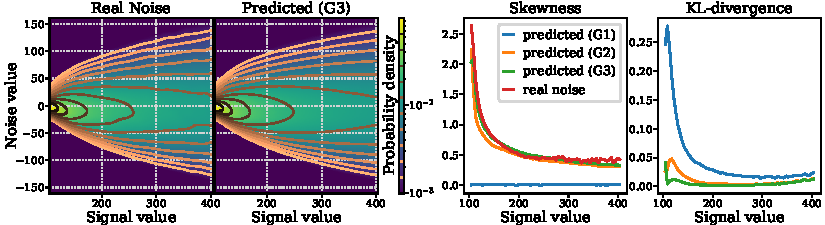
\includegraphics[width=\textwidth]{fig_skewness_1col_w2s-1.pdf}}
\caption{Real noise estimation for dataset \textit{W2S-1}.
The two left graphs represent the empirical distribution of the noise $Y - X$ as a function of $X$ and the corresponding predicted noise distribution for a 3-component-GMM.
The probability density is normalized for each signal value bin.
Skewness of real and predicted noise distribution as a function of $X$, estimated with Pearson's moment coefficient of skewness.
Kullback–Leibler divergence between real noise distribution and predicted distribution generated by each model, as a function of $X$.
\textit{G1} stands for Gaussian model, \textit{G2} for a 2-component-GMM and \textit{G3} a 3-component-GMM.
}
\label{fig:skewness}
\end{center}
\end{figure}

\subsection{Denoising performances}
\label{sec:perf}
\begin{table}[!htbp]
\vskip -0.15in
\caption{Evaluation of our method on 6 datasets with PSNR/SSIM metrics.
SSIM estimates structural similarity (sharpness).
Metrics computed on noisy images are displayed in the \textit{Noisy} column.
The supervised version of our method was not trained for PN2V datasets as they cannot be split into independent train/evaluation sets.
For DecoNoising and N2V, PSNR are taken from \cite{goncharova2020} and SSIM are computed on prediction made by networks trained using the source code provided by the authors (using no positivity constraint, and removing the convolution for N2V).
\textit{Gaussian} corresponds to the optimal Gaussian baseline defined in section~\ref{sec:perf}.
Results for our method predicting a Gaussian model are shown in column \textit{Ours (G1)} (see Table~\ref{si:table:results} for 2/3-component GMM).
Best PSNR $\pm0.1dB$ / SSIM $\pm1\permille$ scores are underlined.}
\label{table:results}
\begin{center}
\begin{small}
\begin{sc}
\resizebox{\textwidth}{!}{
\begin{tabular}{lcccccc}
\toprule
Dataset & Noisy & Gaussian & Supervised & N2V & DecoNoising & Ours (G1) \\
\midrule
PN2V-C & $28.98$ / $0.7713$ & $34.92$ / $0.9409$ & $NA$ / $NA$ & $35.85$ / $0.9404$ & $36.39$ / $0.9483$ & $\underline{38.33}$ / $\underline{0.9754}$ \\
PN2V-MN & $28.10$ / $0.6836$ & $35.53$ / $0.9392$ & $NA$ / $NA$ & $35.86$ / $0.9419$ & $36.34$ / $0.9489$ & $\underline{39.08}$ / $\underline{0.9776}$\\
PN2V-MA & $23.71$ / $0.3731$ & $34.07$ / $0.8739$ & $NA$ / $NA$ & $33.35$ / $0.8384$ & $34.04$ / $0.8633$ & $\underline{34.79}$ / $\underline{0.8905}$\\
W2S-1 & $21.85$ / $0.3490$ & $33.87$ / $0.9326$ & $35.22$ / $0.9608$ & $34.30$ / $0.9026$ & $34.90$ / $0.9169$ & $\underline{35.33}$ / $\underline{0.9619}$\\
W2S-2 & $19.33$ / $0.2256$ & $32.27$ / $0.8531$ & $33.24$ / $0.8828$ & $31.80$ / $0.8311$ & $32.31$ / $0.8524$ & $\underline{33.46}$ / $\underline{0.8867}$\\
W2S-3 & $20.39$ / $0.2232$ & $34.66$ / $0.9013$ & $36.31$ / $0.9252$ & $34.65$ / $0.8637$ & $35.09$ / $0.9051$ & $\underline{36.57}$ / $\underline{0.9263}$\\
\bottomrule
\end{tabular}
}
\end{sc}
\end{small}
\end{center}
\vskip -0.1in
\end{table}

We compared our method to 4 baselines: D-Net trained in a supervised setup with L2 objective (with all other training and prediction hyperparameters unchanged), N2V, DecoNoising, which is the self-supervised blind denoising method that has shown best results on the datasets we considered, as well as one of the most simple denoising method: convolution by a Gaussian, whose standard deviation is chosen to maximizes the PSNR on the evaluation dataset.
We believe the latter makes a good reference, as it is one of the simplest denoising methods, and it removes noise efficiently but also other high-frequency information such as local contrasts.

The considered metrics are summarized in table~\ref{table:results}.
Our method significantly outperforms the baselines both in terms of PSNR and SSIM on all datasets.
For the version predicting a simple Gaussian distribution, the average PSNR gain over DecoNoisng is $+1.42$dB.
This is also confirmed by the visual aspect, displayed in Fig.~\ref{fig:images}: our method produces images closer to the ground truth, smoother, sharper, more detailed and without visual artifacts.
Remarkably, our method performs significantly better than the supervised method CARE \cite{weigert2017content}, with an average PSNR gain of $+1.49$dB (from PSNR values reported in \cite{goncharova2020}).
Moreover, our method also performs better than its supervised counterpart with an average gain of $+0.21$dB (see Table~\ref{si:table:results}).
This could be explained by the fact that self-supervised training induces a lower dependency to central pixel compared to supervised training, and thus pushes the network to make better use of the neighborhood.

\begin{figure}[!htbp]
\vskip -0.1in
\includegraphics[width=\columnwidth]{fig_images.pdf}
\caption{Visual comparison of denoising on the considered datasets. For each dataset a $256$x$256$ portion of an evaluation image is displayed, on which metrics are computed and displayed below. Training of DecoNoising and N2V is described in Table~\ref{table:results}. \textit{Gaussian} corresponds to the optimal Gaussian baseline defined in section~\ref{sec:perf}.}
\label{fig:images}
\end{figure}

To better understand the contribution of the N-Net, we compared our method to the D-Net trained with L2 objective as in \cite{batson2019noise2self, krull2018noise2void}. Table~\ref{si:table:results} shows that adding shows that N-net always improves performances, although not always significantly. Moreover, the addition of the N-net greatly stabilizes the training and improves convergence speed (see Fig.~\ref{si:fig:convergence}), which enables easier hyperparameters and architecture optimization.
From the perspective of our framework, the L2 loss (as used in N2V, N2S) can be understood as a particular case of the N-net predicting a constant unit Gaussian noise. When the actual noise is significantly different from it, the N-net has a stronger impact (e.g. \textit{Speckle} in Fig.~\ref{si:fig:convergence}B).
From a statistical perspective, it is known that considering a sufficiently rich noise model is crucial in deconvolution problem for signal estimation (misspecifying the noise density can lead to very poor deconvolution estimators for instance). This was a motivation to introduce the N-net.
It is worth noting that considering mixture models improves the PSNR in two datasets out of six (Table~\ref{si:table:results}).
As mentioned in Section~\ref{sec:exp:real:noise} an optimal and data-driven choice of the number of components remains an open (and challenging) statistical problem but we believe that such experiments support future research in this direction.

We also ran ablation experiment to better understand the contribution of other aspects of our method, presented in Table~\ref{si:table:ablation}.

\section{Discussion}
\label{sec:discussion}
We introduced a novel self-supervised blind-denoising method modeling both the signal and the noise distributions. We believe its simplicity, performances and the interpretability of the noise distribution will be useful both in practical applications, and as a basis for future research.

First, future works could consider more complex families of noise distributions such as structured or non-centered noises, that can also arise in real-life setups. In particular, \cite{lehtinen2018noise2noise} managed to remove very structured non-centered noises such as overlaid text. With stronger assumptions and architecture changes, it might be possible to capture such noises.

Second, more theoretical works could explore the model proposed in this work  (i) to obtain identifiability of model \eqref{eq:def:Y} and extend \cite{gassiat:lecorff:lehericy:2021} to state-dependent standard deviations and (ii) to establish rates of convergence for the proposed estimators.

Finally, it would also be interesting to understand the role of the central pixel at test time, as it has a significative impact on performance: it depends on the  masking procedure and the convolutional architecture, but the network is not trained explicitly to use it. Our mathematical modeling could be a good basis to study this specific dependency on the central pixel.

% \begin{ack}
% acknowledgments
% \end{ack}
\FloatBarrier
\pagebreak
\bibliographystyle{acm}
\bibliography{blind_denoising}

%
% References follow the acknowledgments. Use unnumbered first-level heading for
% the references. Any choice of citation style is acceptable as long as you are
% consistent. It is permissible to reduce the font size to \verb+small+ (9 point)
% when listing the references.
% Note that the Reference section does not count towards the page limit.

%%%%%%%%%%%%%%%%%%%%%%%%%%%%%%%%%%%%%%%%%%%%%%%%%%%%%%%%%%%%

\section*{Checklist}

\begin{enumerate}

\item For all authors...
\begin{enumerate}
  \item Do the main claims made in the abstract and introduction accurately reflect the paper's contributions and scope?
    \answerYes{}
  \item Did you describe the limitations of your work?
    \answerYes{Section \ref{sec:discussion}}
  \item Did you discuss any potential negative societal impacts of your work?
    \answerNo{Not applicable}
  \item Have you read the ethics review guidelines and ensured that your paper conforms to them?
    \answerTODO{}
\end{enumerate}

\item If you are including theoretical results...
\begin{enumerate}
  \item Did you state the full set of assumptions of all theoretical results?
    \answerNo{Not applicable}
	\item Did you include complete proofs of all theoretical results?
    \answerNo{Not applicable}
\end{enumerate}

\item If you ran experiments...
\begin{enumerate}
  \item Did you include the code, data, and instructions needed to reproduce the main experimental results (either in the supplemental material or as a URL)?
    \answerYes{Section \ref{sec:code}}
  \item Did you specify all the training details (e.g., data splits, hyperparameters, how they were chosen)?
    \answerYes{See \ref{sec:experiments} }
	\item Did you report error bars (e.g., with respect to the random seed after running experiments multiple times)?
    \answerYes{To limit computations, we we verified that all our results are stable. An example of error bar is displayed in Fig. \ref{si:fig:convergence}-D}
	\item Did you include the total amount of compute and the type of resources used (e.g., type of GPUs, internal cluster, or cloud provider)?
    \answerYes{\ref{sec:training}}
\end{enumerate}

\item If you are using existing assets (e.g., code, data, models) or curating/releasing new assets...
\begin{enumerate}
  \item If your work uses existing assets, did you cite the creators?
    \answerYes{\ref{sec:datasets}}
  \item Did you mention the license of the assets?
    \answerNo{No license was found along with the datasets, but they are made publicly available by the authors}
  \item Did you include any new assets either in the supplemental material or as a URL?
    \answerYes{\ref{sec:code}}
  \item Did you discuss whether and how consent was obtained from people whose data you're using/curating?
    \answerYes{Datasets are made publicly available by the authors}
  \item Did you discuss whether the data you are using/curating contains personally identifiable information or offensive content?
    \answerNo{Not applicable}
\end{enumerate}

\item If you used crowdsourcing or conducted research with human subjects...
\begin{enumerate}
  \item Did you include the full text of instructions given to participants and screenshots, if applicable?
    \answerNo{Not applicable}
  \item Did you describe any potential participant risks, with links to Institutional Review Board (IRB) approvals, if applicable?
    \answerNo{Not applicable}
  \item Did you include the estimated hourly wage paid to participants and the total amount spent on participant compensation?
    \answerNo{Not applicable}
\end{enumerate}

\end{enumerate}

%%%%%%%%%%%%%%%%%%%%%%%%%%%%%%%%%%%%%%%%%%%%%%%%%%%%%%%%%%%%

\appendix
\renewcommand{\thetable}{A\arabic{table}}
\renewcommand{\thefigure}{A\arabic{figure}}
\setcounter{table}{0}
\setcounter{figure}{0}
\section{Appendix}


\subsection{Additional Implementation details}
\label{si:implementation}
\subsubsection{Networks and training}
\paragraph{D-Net architecture details.}
The architecture is based on U-net \cite{ronneberger2015u}.
We propose several changes from the original version: we do not crop the image and use zero-padding instead, we use 2 levels of contractions/expansions with 64 filters, expansions are performed by an upsampling layer with nearest-neighbor approximation directly followed by 2x2 convolution. We also add two layers of 1x1 convolution with 64 filters and ReLU activation at the end of the network, and set no activation function at the output layer.

\paragraph{N-Net architecture details.}
In the case of a Gaussian noise, the N-Net is composed 3 successive blocks, each block being composed of two 1x1 convolutions layers of 64 filters, each followed by a non-linear activation layer (alternatively tanh and leaky ReLU with alpha parameter set to $0.1$). A convolution 1x1 with a single channel followed by an exponential activation function is placed after the last block (to ensure that the predicted $\sigma$ is positive).

In the case where the N-net predicts a GMM with N components with weights $(\alpha_i)_{1\leqslant i\leqslant N}$, means $(\mu_i)_{1\leqslant i\leqslant N}$ and variances $(\sigma^2_i)_{1\leqslant i\leqslant N}$, the second block is connected to three distinct blocks, each connected to a convolution 1x1 with:
\begin{itemize}
  \item N channels, followed by an exponential activation function to predict $\sigma_{i}$.
  \item N channels, followed by a softmax activation to predict $\alpha_{i}.$\footnote{When $N=2$, only one channel is used and followed by a sigmoid activation function.}
  \item N-1 channels to predict the distribution means $\mu_{i}$.
\end{itemize}
To ensure that the distribution is centered, the center of the last distribution is computed as
$$
\mu_{N} = - \frac{1}{\alpha_{N}} \sum_{i=1}^{N-1}{\alpha_{i} \mu{i}}\,.
$$

\subsection{Datasets}
\subsubsection{Experimental Datasets}
\label{si:datasetxp}
\paragraph{Datasets published along with the PN2V \cite{krull2019probabilistic}.}
\begin{itemize}
  \item \emph{Convallaria} dataset, referred to as \emph{PN2V-C} is composed of 100 images of size $1024$x$1024$. Evaluation subset is: $Y\in\interval{0}{512}, X\in\interval{0}{512}$.
  \item \emph{Mouse skull nuclei} referred to as \emph{PN2V-MN} is composed 200 images of size $512$x$512$. Evaluation subset is: $Y\in\interval{0}{512}, X\in\interval{0}{256}$.
  \item \emph{Mouse Actin} referred to as \emph{PN2V-MA} is composed of 100 images of size $1024$x$1024$. Evaluation subset is: $Y\in\interval{0}{1024}, X\in\interval{0}{512}$.
\end{itemize}

The \emph{PN2V-C} and \emph{PN2V-MA} datasets are acquired on a spinning disc confocal microscope and \emph{PN2V-MN} dataset is acquired with a point scanning confocal microscope.
Datasets can be downloaded from: \url{https://github.com/juglab/pn2v}

We observed that datasets acquired with a spinning disc confocal microscope display axial noise correlation (see \ref{sec:datasets}).

\paragraph{Datasets published in \cite{zhou2020w2s}.}

We used the 16-bit raw images kindly provided by the authors.
The dataset is composed of 120 FOV of 400 observations of size $512$x$512$ pixels.
The first 80 are used for training and the last 40 for evaluation.
Following the authors, for each FOV, only the observation of index 249 is used for training and evaluation
images are acquired with a electron-multiplying charge-coupled device camera on a wide-field microscope.
It can be downloaded here: \url{https://datasets.epfl.ch/w2s/W2S_raw.zip}

\paragraph{Normalization.}

For both datasets images were normalized using the modal value as center and the difference between modal value and $95\%$ percentile as scale factor, computed on the whole dataset.
This is relevant in fluorescence microscopy data where signal is often less abundant than background with proportion that vary among images and signal distribution often has a heavy tail towards high values.

\paragraph{Metrics.}
For the 6 chosen datasets, images are encoded in 16-bit.
PSNR is defined as $PSNR = 10 \log_{10}(d/\mathrm{MSE})$, with $d$ the maximum possible pixel value of the image and $\mathrm{MSE}$ the mean squared error.
For 8-bit encoded images d is simply $255$, and for 16-bit images it would be $65635$ but this does not correspond to the actual possible range of microscopy data, thus the actual range of values of each ground truth image is used. This is also what is done in \cite{goncharova2020} as we obtain the same PSNR values for raw images.
The same applies for SSIM computation.

\subsubsection{Synthetic noise datasets}
\label{si:synthetic}
\begin{itemize}
  \item Additive Gaussian: $Y = X + \varepsilon$ with $\varepsilon \sim \mathcal{N}(0, \sigma^2)$, $\sigma=20$.
  \item Poisson-Gaussian: $Y = X + (\alpha * (X-\underline{X}) + \eta^2 )^{1/2}\varepsilon$  with $\varepsilon \sim \mathcal{N}(0, 1)$, $\alpha=5, \eta=12$ and $\underline{X}$ being the minimal value of the ground truth on the whole dataset.
  \item Speckle: $X = X + (X-\underline{X})\varepsilon$  with $\varepsilon \sim \mathcal{N}(0, \sigma^2)$, $\sigma=0.405$ and $\underline{X}$ being the minimal value of the ground truth on the whole dataset.
\end{itemize}

\subsection{Impact of N-Net}
\begin{figure}[ht]
\begin{center}
\centerline{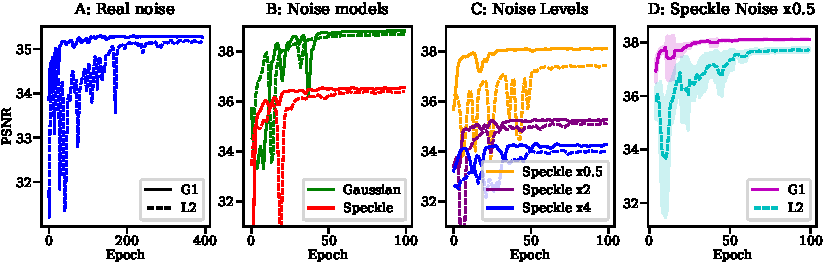
\includegraphics[width=\columnwidth]{fig_convergence_1col.pdf}}
\caption{PSNR at each epoch on the test set for N-net (G1) or D-net only (L2). A: training on real noise. B, C: training on different models/levels of synthetic noise added to ground truth image. B: \textit{Gaussian} and \textit{Speckle} correspond to noises presented in 5.1, that have no and high signal dependency respectively. C: \textit{Speckle} with variance multiplied by 0.5, 2 and 4. D: Mean and SEM over 5 runs.}
\label{si:fig:convergence}
\end{center}
\end{figure}

\begin{table}[ht]
\caption{Evaluation of the impact of N-Net on performances with PSNR/SSIM metrics. Comparison between our method predicting a GMM with 1, 2, or 3 components (respectively G1, G2, G3) and D-Net only trained with L2 loss (with training and prediction scheme unchanged).
Best PSNR $\pm0.1dB$ / SSIM $\pm1\permille$ scores are underlined.}
\label{si:table:results}
\begin{center}
\begin{sc}
\begin{tabular}{lccccc}
\toprule
Dataset & Noisy & Ours (L2) & Ours (G1) & Ours (G2) & Ours (G3) \\
\midrule
PN2V-C & $28.98$ / $0.7713$ & $38.23$ / $0.9729$ & $38.33$ / $\underline{0.9754}$ & $\underline{38.47}$ / $0.9738$ & $38.28$ / $\underline{0.9756}$ \\
PN2V-MN & $28.10$ / $0.6836$ & $39.08$ / $0.9747$ & $39.08$ / $\underline{0.9776}$ & $\underline{39.22}$ / $\underline{0.9779}$ & $\underline{39.18}$ / $\underline{0.9780}$ \\
PN2V-MA & $23.71$ / $0.3731$ & $34.63$ / $0.8890$ & $\underline{34.79}$ / $\underline{0.8905}$ & $34.68$ / $0.8880$ & $\underline{34.70}$ / $0.8877$ \\
W2S-1 & $21.85$ / $0.3490$ & $\underline{35.23}$ / $0.9611$ & $\underline{35.33}$ / $\underline{0.9619}$ & $\underline{35.27}$ / $\underline{0.9623}$ & $\underline{35.27}$ / $\underline{0.9624}$ \\
W2S-2 & $19.33$ / $0.2256$ & $\underline{33.44}$ / $0.8860$ & $\underline{33.46}$ / $\underline{0.8867}$ & $\underline{33.48}$ / $\underline{0.8871}$ & $\underline{33.47}$ / $\underline{0.8871}$ \\
W2S-3 & $20.39$ / $0.2232$ & $\underline{36.56}$ / $\underline{0.9263}$ & $\underline{36.57}$ / $\underline{0.9263}$ & $\underline{36.60}$ / $\underline{0.9269}$ & $\underline{36.59}$ / $\underline{0.9269}$ \\
\bottomrule
\end{tabular}
\end{sc}
\end{center}
\end{table}
\FloatBarrier

\subsection{Ablation experiments}
To better understand the contribution of different aspects of our method, we ran ablation experiment, presented in Table~\ref{si:table:ablation}
\begin{table}[ht]
\caption{Ablation experiment on dataset W2S-1, with PSNR/SSIM metrics.
\textit{No Invariance}: removed averaging with flipped and transposed images.
\textit{N2V Masking}: masking scheme used in N2V (random points and replacement by a random neighbor). \textit{Transpose Convolution}: D-Net architecture is modified: nearest-neighbor upsampling and 2x2 convolution are replaced by a transpose convolution. }
\label{si:table:ablation}
\begin{center}
\begin{sc}
\begin{tabular}{lccccc}
\toprule
Ours (G1) & No Invariance & N2V Masking & Transpose Convolution \\
\midrule
$35.33$ / $0.9619$ & $35.28$ / $0.9608$ & $NA$ / $NA$ & $NA$ / $NA$ \\
\bottomrule
\end{tabular}
\end{sc}
\end{center}
\end{table}

\FloatBarrier
\subsection{Noise estimation}
\label{si:skewness}
This section contains the figures corresponding to Fig~\ref{fig:skewness} for each dataset.
Note that they are computed using regular signal value bins and excluding signal values greater to the $99.5\%$ percentile of the dataset so that there are enough observed samples in each bin to compute statistically significant metrics.

\begin{figure}[ht]
\begin{center}
\centerline{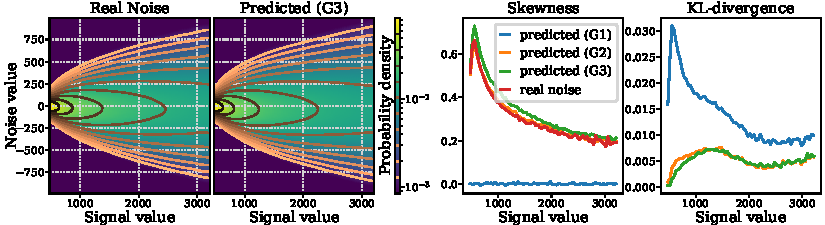
\includegraphics[width=\columnwidth]{fig_skewness_1col_pn2v-C.pdf}}
\caption{Real noise estimation for dataset \textit{PN2V-C}. See main text Fig~\ref{fig:skewness}.
}
\end{center}
\end{figure}

\begin{figure}[ht]
\begin{center}
\centerline{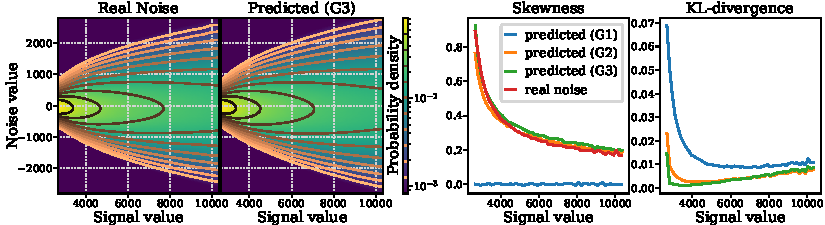
\includegraphics[width=\columnwidth]{fig_skewness_1col_pn2v-MN.pdf}}
\caption{Real noise estimation for dataset \textit{PN2V-MN}. See main text Fig~\ref{fig:skewness}.
}
\end{center}
\end{figure}

\begin{figure}[ht]
\begin{center}
\centerline{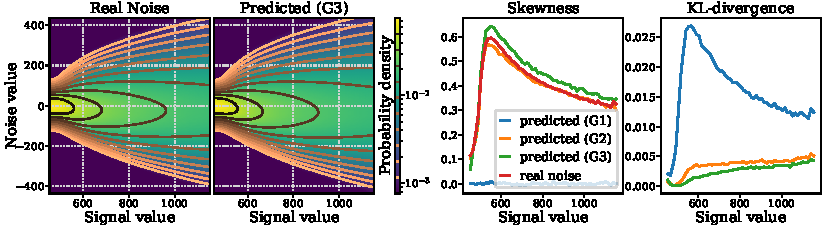
\includegraphics[width=\columnwidth]{fig_skewness_1col_pn2v-MA.pdf}}
\caption{Real noise estimation for dataset \textit{PN2V-MA}. See main text Fig~\ref{fig:skewness}.
}
\end{center}
\end{figure}

\begin{figure}[ht]
\begin{center}
\centerline{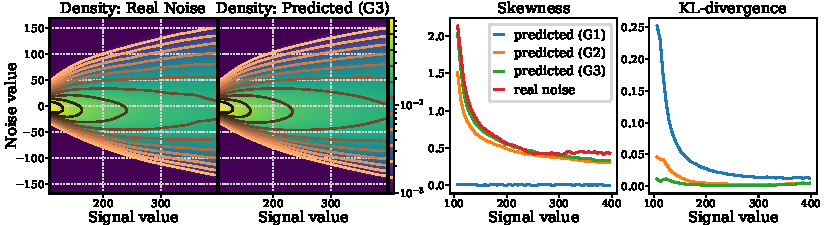
\includegraphics[width=\columnwidth]{fig_skewness_1col_w2s-2.pdf}}
\caption{Real noise estimation for dataset \textit{W2S-2}. See main text Fig~\ref{fig:skewness}.
}
\end{center}
\end{figure}

\begin{figure}[ht]
\begin{center}
\centerline{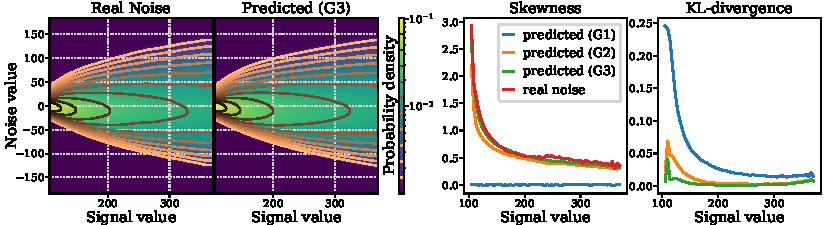
\includegraphics[width=\columnwidth]{fig_skewness_1col_w2s-3.pdf}}
\caption{Real noise estimation for dataset \textit{W2S-3}. See main text Fig~\ref{fig:skewness}.
}
\end{center}
\end{figure}
\FloatBarrier
\subsection{Code}
\label{sec:code}
Source code can be found at this url: \url{https://github.com/code-ssbd/ssbd}.
A ready-to-use google colab notebook that includes training and evaluation procedures can be found at this address: \url{https://gist.github.com/code-ssbd/9cbdeb6f4b9912514b5b8afb962e9276} by clicking on the \textit{open in colab} banner. To execute it a google account is required.


% {\small
% \bibliographystyle{acm}
% \bibliography{blind_denoising}
%
% }

\end{document}
